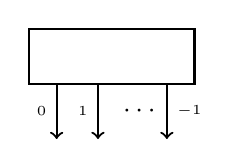
\begin{tikzpicture}[scale=0.35,thick] % , baseline = -3.5pt


\draw (-1,-1) rectangle (5,-3);
\node[anchor=center] (text) at (2,-2) {\small $\probtensor$};
\draw[->] (0,-3)--(0,-5) node[midway,left] {\tiny $\catvariableof{0}$};
\draw[->] (1.5,-3)--(1.5,-5) node[midway,left] {\tiny $\catvariableof{1}$};
\node[anchor=center] (text) at (3,-4) {$\cdots$};
\draw[->] (4,-3)--(4,-5) node[midway,right] {\tiny $\catvariableof{\atomorder-1}$};

%\drawatomcore{3.5}{-8}{$\probtensor$}
%\drawatomindices{3.5}{-12}	
%\draw (5.5,-9)--(5.5,-7) node[midway,right] {\tiny $\catvariableof{\exformula}$};

\end{tikzpicture}